%!TEX root=../document.tex
\lstset{
  basicstyle=\ttfamily,
  columns=fullflexible,
  showstringspaces=false,
  commentstyle=\color{gray}\upshape
}

\lstdefinelanguage{XML}
{
  morestring=[b]",
  morestring=[s]{>}{<},
  morecomment=[s]{<?}{?>},
  stringstyle=\color{black},
  identifierstyle=\color{darkblue},
  keywordstyle=\color{cyan},
  morekeywords={xmlns,version,type}% list your attributes here
}

\section{Einf�hrung}

\subsection{Ziele}
Erstes Ann�hern an XML.

\subsection{Voraussetzungen}

\subsection{Aufgabenstellung}

\begin{enumerate}
	\item Erstelle ein XML-Dokument f�r die 4AHITM.
	\item Welche Daten speicherst du als Attribut oder Element?
	\item Erstelle 5 Testpersonen
	\item Einbau von Elementen und Attributen
	\item �berpr�fung auf Wohlgeformheit durch Tool
	\item Stelle dein Ergebnis als DOM - Baum dar.
	\item Erweiterung 1 : Erstelle und beschreibe f�nf unterschiedliche Beispiele, welche die Wohlgeformtheit verletzen und erkl�re die verletzte Regel.
	\item Erweiterung 2 : Schreibe ein kleines Java-Programm, welches die Wohlgeformtheit einer konfigurierbaren XML-Datei �berpr�ft.
\end{enumerate}

\clearpage

\section{Code}
Folgende Punkte werden hier bearbeitet:
\begin{itemize}
	\item Erstelle ein XML-Dokument f�r die 4AHITM.
	\item Erstelle mind. 5 Testpersonen
	\item Einbau von Elementen und Attributen
\end{itemize}

\lstset{language=XML}
\begin{lstlisting}
<?xml version="1.0" encoding="UTF-8" standalone="no" ?>
<class id="4AHITM" count="24">
  <classmember sex="m" can_type_10_fingers="true">
    <name>Lorenz Breier</name>
    <fav_meal>Topfenhaluski</fav_meal>
    <best_subject>Religion</best_subject>
    <eye_color>blau</eye_color>
    <fav_gen>Jazz</fav_gen>
    <computer>Apple Macbook</computer>
  </classmember>

  <classmember sex="m" can_type_10_fingers="false">
    <name>Dominik Wojdyla</name>
    <fav_meal>Nicht vorhanden</fav_meal>
    <best_subject>Turnen</best_subject>
    <eye_color>gr�n-blau</eye_color>
    <fav_gen>Indie</fav_gen>
    <computer>Apple Macbook</computer>
  </classmember>

  <classmember sex="m" can_type_10_fingers="false">
    <name>Jakob Greimel</name>
    <fav_meal>Hauptsache irgendwas ohne Fleisch</fav_meal>
    <best_subject>Freistunde</best_subject>
    <eye_color>braun</eye_color>
    <fav_gen>Rock</fav_gen>
    <computer>Acer</computer>
  </classmember>


  <classmember sex="m" can_type_10_fingers="false">
    <name>Matthias Mischek</name>
    <fav_meal>Pizza</fav_meal>
    <best_subject>Turnen</best_subject>
    <eye_color>braun</eye_color>
    <fav_gen>Indie</fav_gen>
    <computer>Apple Macbook</computer>
  </classmember>

  <classmember sex="m" can_type_10_fingers="false">
    <name>Matthias Stickler</name>
    <fav_meal>Kaiserschmarrn</fav_meal>
    <best_subject>Medientechnik</best_subject>
    <eye_color>braun</eye_color>
    <fav_gen>Drum'n Bass</fav_gen>
    <computer>Hewlett Packard</computer>
  </classmember>

  <classmember sex="m" can_type_10_fingers="false">
    <name>Moritz Netrwal</name>
    <fav_meal>schwer-zu-sagen-Suppe</fav_meal>
    <best_subject>ITP2</best_subject>
    <eye_color>braun</eye_color>
    <fav_gen>Gamemusic</fav_gen>
    <computer>Alienware</computer>
  </classmember>

</class>
\end{lstlisting}

\section{Welche Daten speicherst du als Attribut oder Element?}
Das ist Geschmackssache. Handelt es sich um nur kurze Infromationen, ist es sinnvoll diese einfach als Attribut hinzuzuf�gen.
Um das Ganze zu veranschaulichen, habe ich ein Beispiel von w3schools genommmen, und bisschen auch ver�ndert, um den Einsatz deutlicher zu machen.
Beispiel:
\begin{lstlisting}
<person sex="f" age="42" student="true">
  <firstname>Anna</firstname>
  <lastname>Smith</lastname>
  <description>Anna is a really nice person. She likes to play music and to eat sweets on the roof.</description>
</person>
\end{lstlisting}

Als Gegenbeispiel bietet w3schools einen sch�nen Code. Sein / Ihr Kommentar "Don't end up like this: ".
\begin{lstlisting}
<note day="10" month="01" year="2008"
to="Tove" from="Jani" heading="Reminder"
body="Don't forget me this weekend!">
</note>
\end{lstlisting}

\section{�berpr�fung auf Wohlgeformheit durch Tool}
\subsection{mit Hilfe von validome.org}
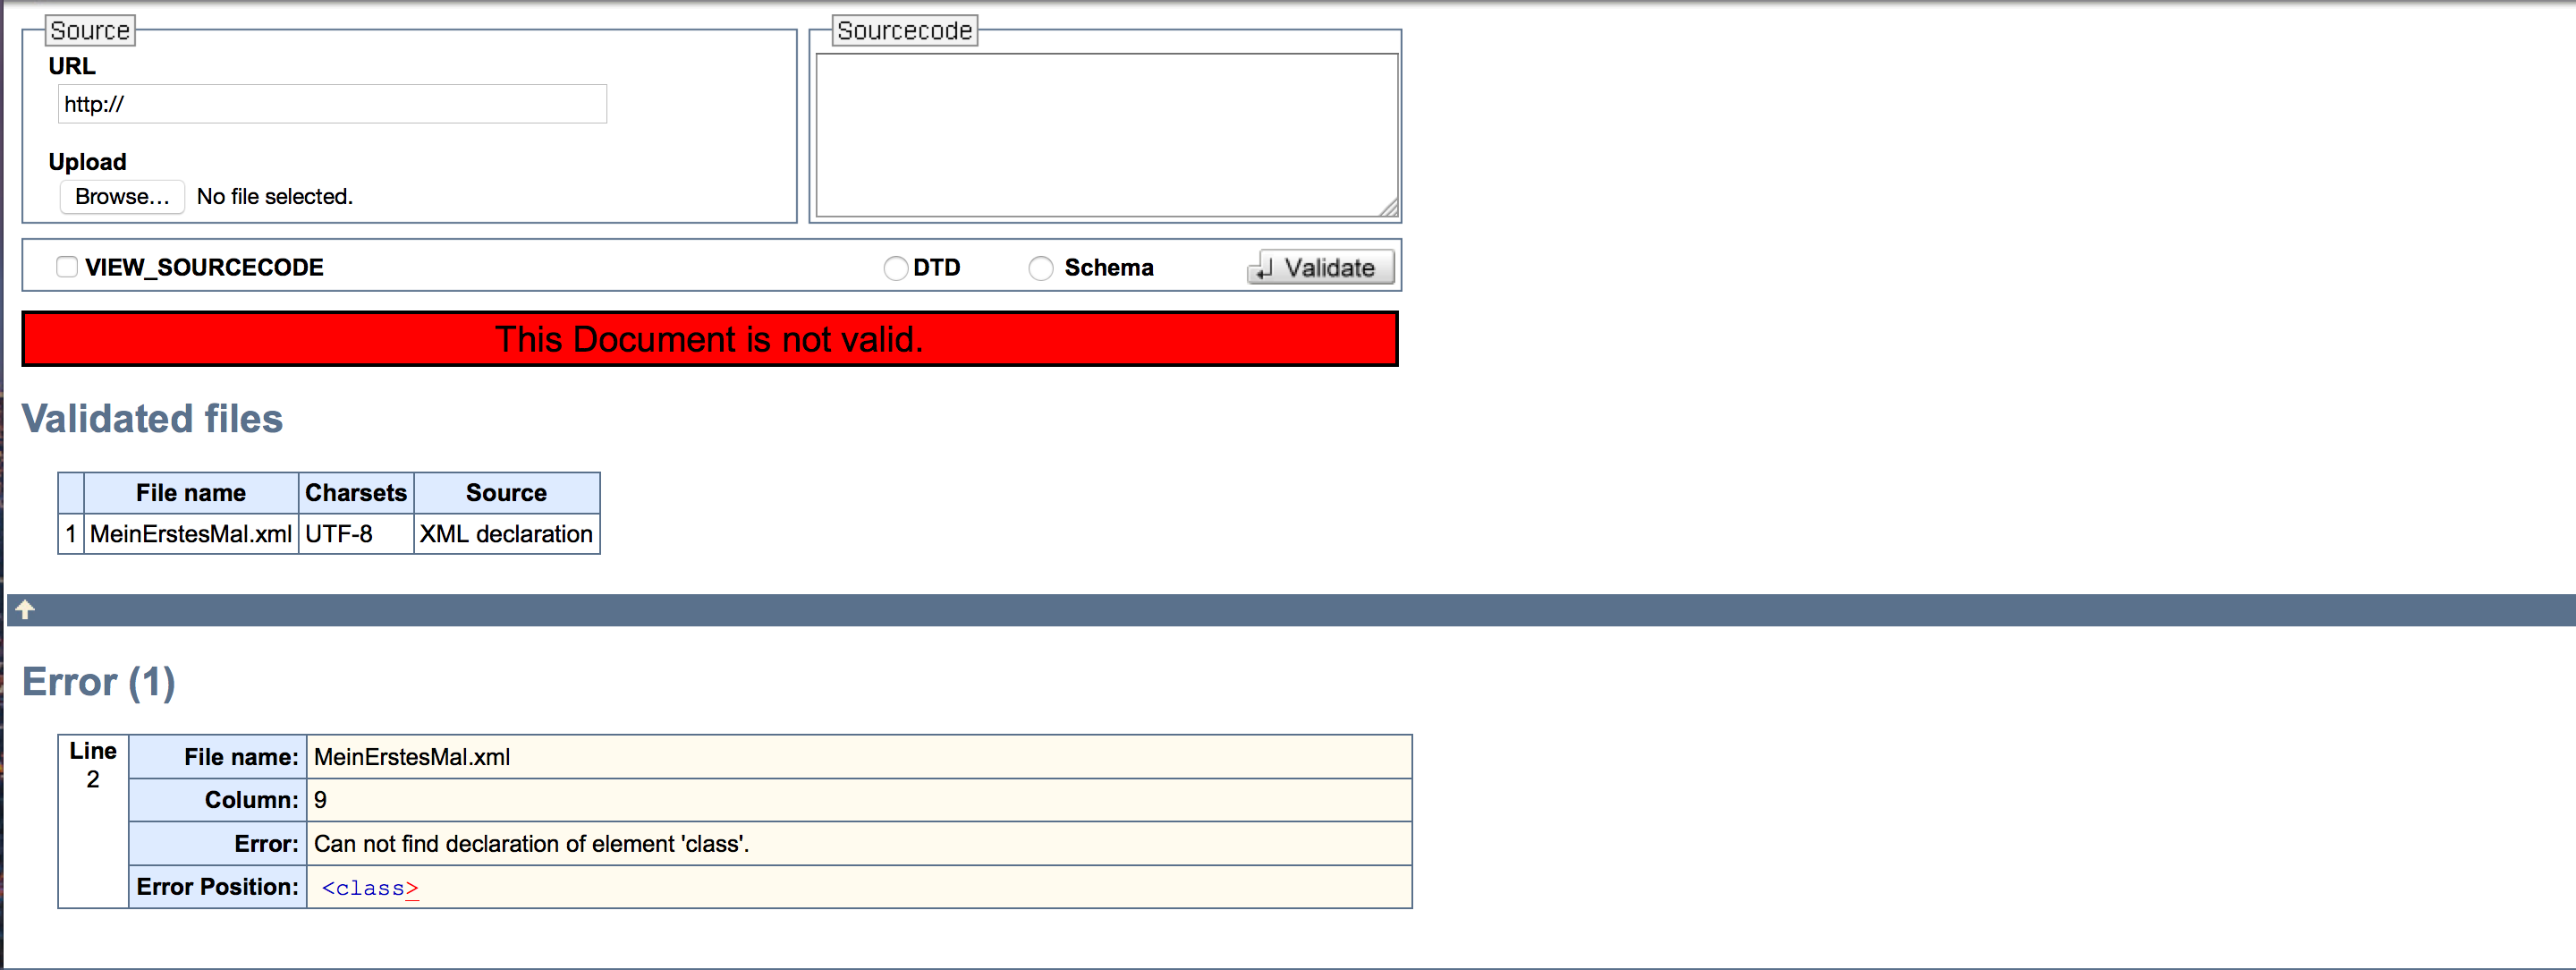
\includegraphics[scale=0.35]{images/validome.png}
validome sagt, wir haben einen Fehler.
"Offensichtlich sucht er nach einem SCHEMA", sagt Professor Dolezal, w�hrend er sicht dabei das Kinn herunterf�hrt.
Daraufhin r�t er mir, ich solle doch den w3schools - Validator zum �berpr�fen nutzen. Warum w3schools?
Ganz einfach, weil w3schools im Netz einfach DER Validator ist.

\subsection{mit Hilfe von w3schools.com}
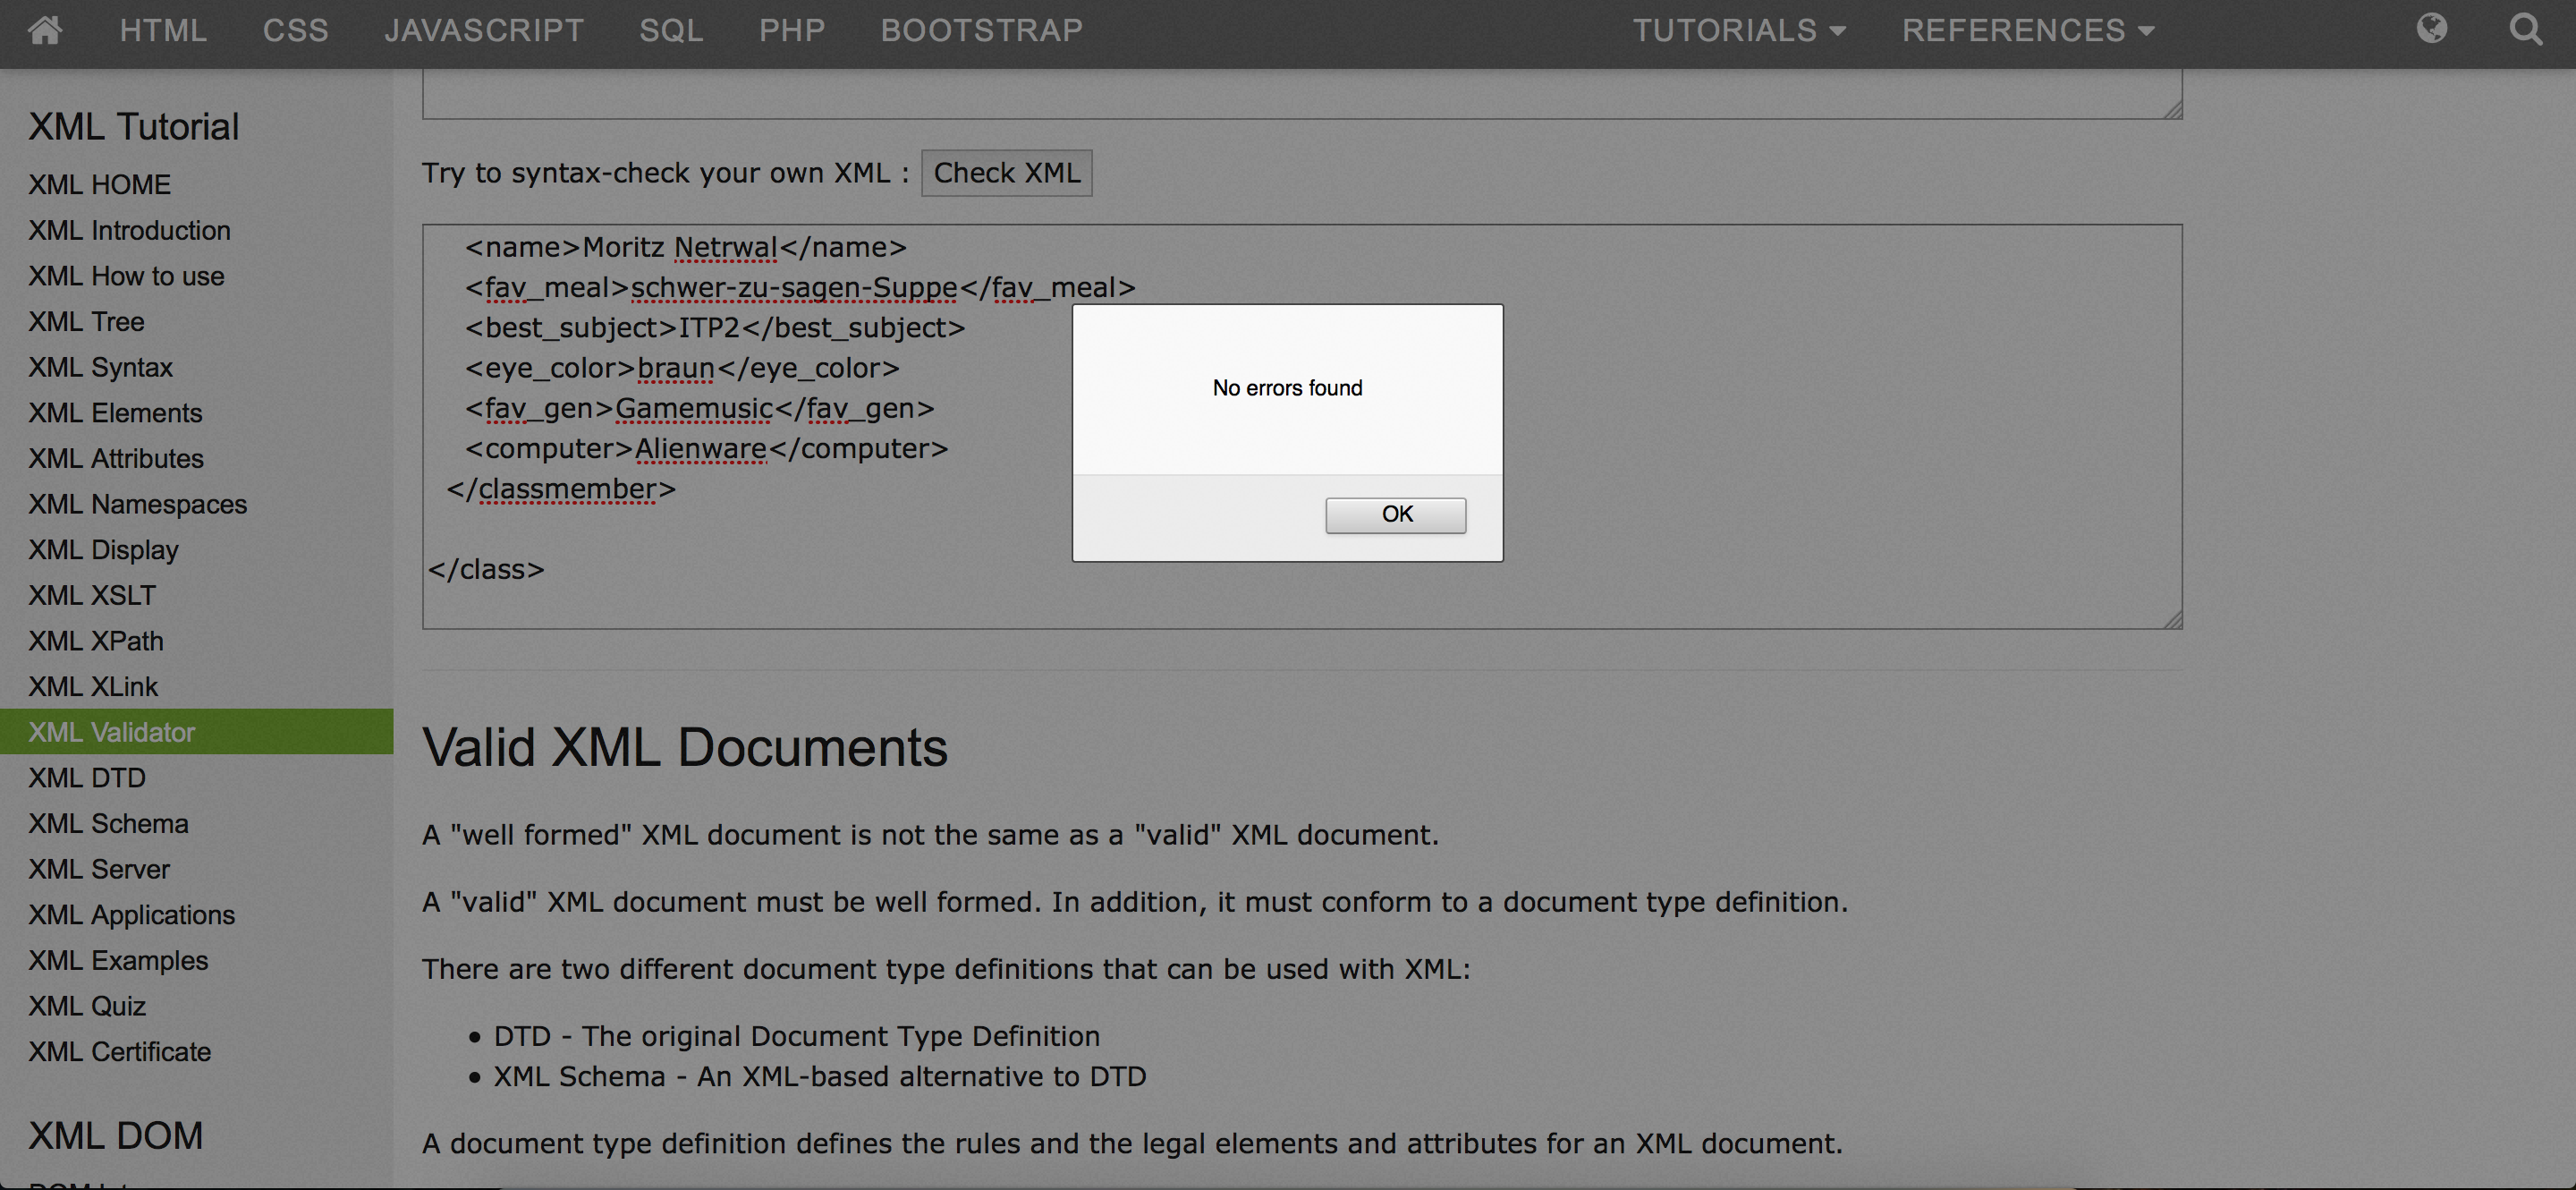
\includegraphics[scale=0.35]{images/w3schools.png}
Wie man sehn kann : der w3schools - Editor wirft keine Fehler.

\section{DOM - Baum Grafik}
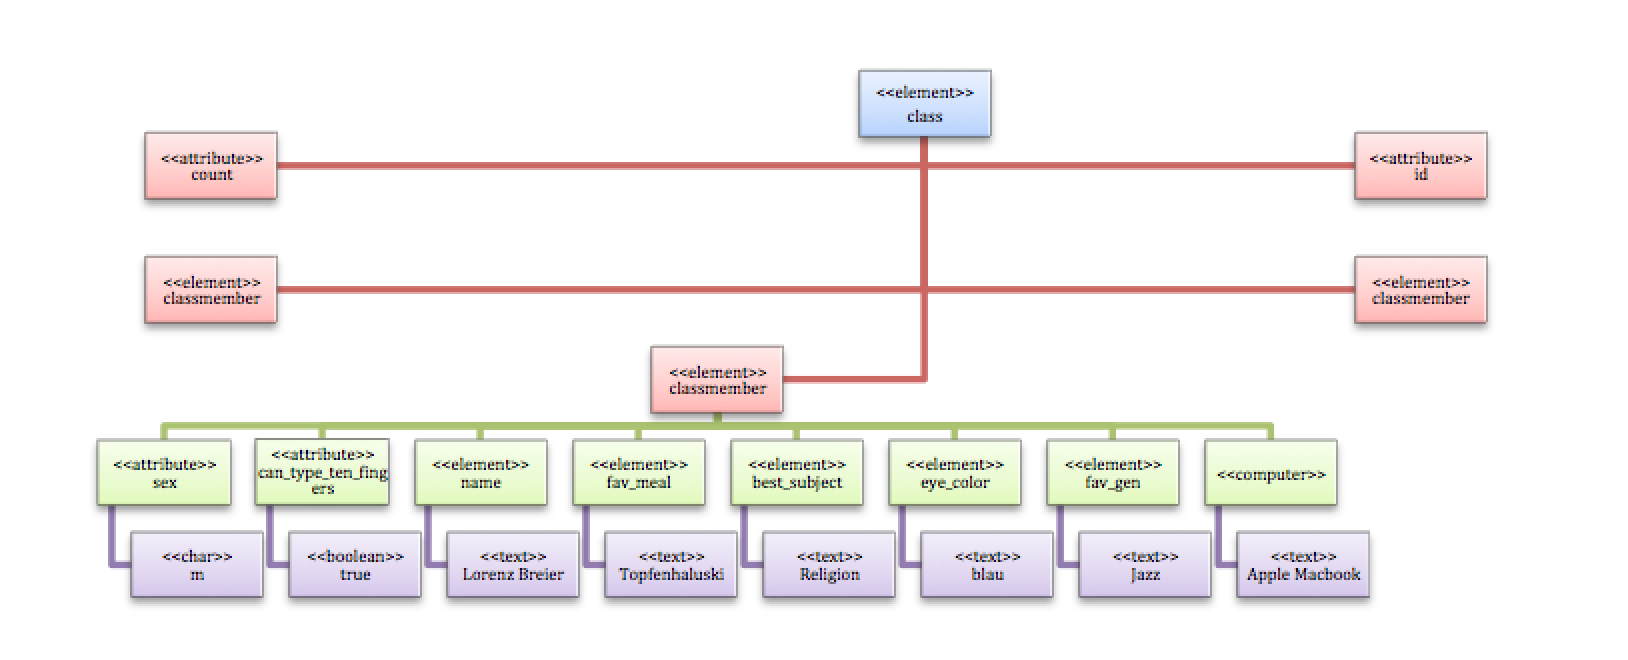
\includegraphics[scale=0.7]{images/d.png}


\section{Pl�doyer}
XML ist eine Auszeichnungssprache, welche f�r Serialisierungen und zum Transportieren von Informationen verwendet wird. Beispielsweise k�nnte ein Notizen-Programm seine Notizen in einer XML - Datei ablegen. So kann man diese XML - File einfach verschicken und auf einem anderen Rechner unter dem selben Programm �ffnen. \\
XML - Files haben den Vorteil, dass sie eine strukturierte Darstellung haben, und deswegen "menschenlesbar" sind.
XML - Files werden gerne f�r Webapplikationen verwendet, und mittels DOM werden auf XML - Dateien zugegriffen.

